\documentclass[11pt]{article}
\usepackage[a4paper,margin=2cm]{geometry}
\usepackage{booktabs}
\usepackage{graphicx}
\usepackage{adjustbox}
\begin{document}
\begin{table}[htbp]
\centering
\footnotesize
\caption{Feature-based detectors, clean training (test set, family-weighted).}
\label{tab:baselines}
\begin{adjustbox}{max width=\linewidth}
\begin{tabular}{lcccc}
\toprule
Detector & ROC-AUC [95\% CI] & Caught (\%) [95\% CI] & Conn. AUC & Iso. AUC \\
\midrule
\multicolumn{5}{l}{\textit{Features: static + dependencies + names, without GuardDog}} \\
Isolation Forest & 0.895 [0.884, 0.905] & 20.1 [8.0, 28.5] & 0.815 & 0.940 \\
LOF & 0.890 [0.878, 0.902] & 37.4 [32.7, 44.5] & 0.809 & 0.917 \\
One-Class SVM & 0.929 [0.920, 0.937] & 57.3 [43.3, 60.9] & 0.867 & 0.946 \\
One-Class SVM, per-group thresholds & 0.927 [0.918, 0.936] & 58.8 [54.9, 62.7] & 0.868 & 0.946 \\
\multicolumn{5}{l}{\textit{Features: static + dependencies + names, with GuardDog}} \\
Isolation Forest & 0.944 [0.936, 0.952] & 43.2 [27.4, 56.6] & 0.900 & 0.968 \\
LOF & 0.914 [0.903, 0.923] & 43.7 [40.6, 46.8] & 0.848 & 0.933 \\
One-Class SVM & 0.963 [0.957, 0.969] & 73.9 [70.6, 76.8] & 0.935 & 0.971 \\
One-Class SVM, per-group thresholds & 0.962 [0.956, 0.968] & 74.6 [71.1, 77.4] & 0.935 & 0.971 \\
\midrule
GuardDog rule (any rule fires) & 0.902 [0.890, 0.913] & -- & 0.808 & 0.936 \\
Random Forest, supervised (reference) & 0.986 [0.981, 0.990] & 90.6 [87.7, 92.3] & 0.966 & 0.993 \\
\bottomrule
\end{tabular}
\end{adjustbox}
\par\smallskip
\parbox{0.95\linewidth}{\footnotesize Settings chosen on validation (pAUC up to 5\% FPR). Caught: family-weighted share of malware flagged at a 1\% false-positive rate. Connected / isolated: packages with / without dependency relations to the training graph. Scores of the 3 seeds are rank-averaged (ensemble); the One-Class SVM is deterministic, so its seeds coincide. The supervised reference uses labelled malware and is not comparable to the unsupervised detectors.}
\end{table}

\begin{table}[htbp]
\centering
\small
\caption{Feature-based detectors under contamination: ROC-AUC / caught at 1\% FPR (\%, mean over 3 contamination draws).}
\label{tab:baselines-contam}
\begin{tabular}{lcccc}
\toprule
Detector & 0\% & 1\% & 2\% & 5\% \\
\midrule
Isolation Forest & 0.944 / 41.2 & 0.946 / 53.8 & 0.944 / 49.2 & 0.938 / 30.0 \\
LOF & 0.914 / 43.7 & 0.605 / 15.2 & 0.556 / 15.5 & 0.589 / 19.8 \\
One-Class SVM & 0.963 / 73.9 & 0.951 / 34.9 & 0.944 / 17.9 & 0.928 / 9.1 \\
One-Class SVM, per-group & 0.962 / 74.6 & 0.953 / 62.6 & 0.947 / 37.7 & 0.920 / 8.2 \\
\bottomrule
\end{tabular}
\par\smallskip
\parbox{0.95\linewidth}{\footnotesize All features including GuardDog. Contamination: share of unlabelled malware in the training set.}
\end{table}

\begin{table}[htbp]
\centering
\small
\caption{CoLA (re-implemented, inductive protocol): ROC-AUC below 0.5 means malware is ranked as more normal than normal packages.}
\label{tab:cola}
\begin{adjustbox}{max width=\linewidth}
\begin{tabular}{llcccc}
\toprule
Contam. & Variant & ROC-AUC [95\% CI] & Caught (\%) & Connected AUC & Isolated AUC \\
\midrule
0\% & CoLA 1-hop (p2=0.0) & 0.197 [0.179, 0.216] & 1.3 & 0.501 & 0.133 \\
0\% & CoLA (p2=1.0) & 0.233 [0.215, 0.252] & 2.7 & 0.472 & 0.329 \\
1\% & CoLA 1-hop (p2=0.0) & 0.188 [0.172, 0.205] & 1.4 & 0.425 & 0.159 \\
2\% & CoLA 1-hop (p2=0.0) & 0.175 [0.160, 0.191] & 1.0 & 0.347 & 0.167 \\
5\% & CoLA 1-hop (p2=0.0) & 0.170 [0.155, 0.185] & 1.0 & 0.340 & 0.150 \\
\bottomrule
\end{tabular}
\end{adjustbox}
\end{table}

\begin{table}[htbp]
\centering
\footnotesize
\caption{Contrastive encoders with tuned training settings (validation-chosen depth and scorer).}
\label{tab:contrastive-tuned}
\begin{adjustbox}{max width=\linewidth}
\begin{tabular}{lllcccc}
\toprule
Loss & Encoder & Chosen & ROC-AUC & Caught (\%) & Conn. AUC & Iso. AUC \\
\midrule
\multicolumn{7}{l}{\textit{Contamination 0\%}} \\
InfoNCE & GIN & OCSVM, depth 1 & 0.964 & 65.6 $\pm$ 10.9 & 0.935 & 0.966 \\
InfoNCE & GAT & OCSVM, depth 2 & 0.962 & 71.5 $\pm$ 0.3 & 0.926 & 0.969 \\
InfoNCE & TransformerConv & OCSVM, depth 2 & 0.962 & 71.4 $\pm$ 0.4 & 0.930 & 0.966 \\
InfoNCE & GraphGPS & OCSVM, depth 1 & 0.963 & 67.2 $\pm$ 9.7 & 0.934 & 0.968 \\
Triplet & GIN & OCSVM, depth 1 & 0.962 & 74.3 $\pm$ 1.6 & 0.925 & 0.970 \\
Triplet & GAT & OCSVM, depth 2 & 0.953 & 67.3 $\pm$ 1.6 & 0.910 & 0.967 \\
Triplet & TransformerConv & OCSVM, depth 1 & 0.958 & 73.3 $\pm$ 1.2 & 0.919 & 0.966 \\
Triplet & GraphGPS & OCSVM, depth 1 & 0.963 & 73.8 $\pm$ 0.4 & 0.927 & 0.969 \\
DGI & GIN & OCSVM, depth 1 & 0.962 & 74.5 $\pm$ 1.4 & 0.921 & 0.973 \\
DGI & GAT & OCSVM, depth 1 & 0.960 & 73.3 $\pm$ 1.9 & 0.913 & 0.973 \\
DGI & TransformerConv & OCSVM, depth 1 & 0.959 & 73.0 $\pm$ 1.8 & 0.919 & 0.970 \\
DGI & GraphGPS & OCSVM, depth 1 & 0.962 & 72.1 $\pm$ 1.4 & 0.920 & 0.974 \\
\multicolumn{3}{l}{Raw One-Class SVM (reference)} & 0.963 & 73.9 & 0.935 & 0.971 \\
\multicolumn{7}{l}{\textit{Contamination 1\%}} \\
InfoNCE & GIN & OCSVM, depth 1 & 0.941 & 38.8 $\pm$ 11.0 & 0.898 & 0.946 \\
InfoNCE & GAT & OCSVM, depth 2 & 0.933 & 32.0 $\pm$ 5.4 & 0.884 & 0.945 \\
InfoNCE & TransformerConv & OCSVM, depth 2 & 0.931 & 21.0 $\pm$ 3.3 & 0.886 & 0.938 \\
InfoNCE & GraphGPS & OCSVM, depth 1 & 0.930 & 40.2 $\pm$ 10.5 & 0.868 & 0.948 \\
Triplet & GIN & OCSVM, depth 1 & 0.938 & 30.0 $\pm$ 1.3 & 0.904 & 0.929 \\
Triplet & GAT & OCSVM, depth 2 & 0.930 & 55.0 $\pm$ 11.7 & 0.861 & 0.948 \\
Triplet & TransformerConv & OCSVM, depth 1 & 0.941 & 52.4 $\pm$ 12.4 & 0.892 & 0.952 \\
Triplet & GraphGPS & OCSVM, depth 2 & 0.937 & 16.7 $\pm$ 1.2 & 0.911 & 0.923 \\
DGI & GIN & OCSVM, depth 1 & 0.950 & 50.6 $\pm$ 19.5 & 0.898 & 0.963 \\
DGI & GAT & OCSVM, depth 1 & 0.947 & 54.5 $\pm$ 9.8 & 0.883 & 0.964 \\
DGI & TransformerConv & OCSVM, depth 1 & 0.947 & 55.9 $\pm$ 11.1 & 0.902 & 0.960 \\
DGI & GraphGPS & IF, depth 1 & 0.947 & 51.8 $\pm$ 14.2 & 0.886 & 0.965 \\
\multicolumn{3}{l}{Raw One-Class SVM (reference)} & 0.951 & 34.9 $\pm$ 1.7 & 0.921 & 0.963 \\
\bottomrule
\end{tabular}
\end{adjustbox}
\par\smallskip
\parbox{0.95\linewidth}{\footnotesize Caught: mean $\pm$ sd over 3 training seeds. ROC-AUC: rank-averaged seed ensemble.}
\end{table}

\begin{table}[htbp]
\centering
\small
\caption{Capacity check: depth-1 embeddings are twice as large (own-feature projection + neighbourhood). Giving the no-graph model the same size removes most of the graph's apparent gain.}
\label{tab:capacity}
\begin{adjustbox}{max width=\linewidth}
\begin{tabular}{llcccc}
\toprule
Loss & Model (One-Class SVM scorer) & ROC-AUC & Caught (\%) & Connected AUC & Isolated AUC \\
\midrule
InfoNCE & No graph, tuned size & 0.934 & 71.2 & 0.882 & 0.951 \\
InfoNCE & No graph, size 128 & 0.940 & 63.8 & 0.897 & 0.953 \\
InfoNCE & GIN depth 1, tuned size & 0.964 & 65.6 & 0.935 & 0.966 \\
\addlinespace
Triplet & No graph, tuned size & 0.953 & 66.2 & 0.917 & 0.963 \\
Triplet & No graph, size 256 & 0.955 & 73.2 & 0.921 & 0.966 \\
Triplet & GIN depth 1, tuned size & 0.962 & 74.3 & 0.925 & 0.970 \\
\addlinespace
DGI & No graph, tuned size & 0.952 & 70.2 & 0.913 & 0.967 \\
DGI & No graph, size 256 & 0.958 & 73.2 & 0.918 & 0.973 \\
DGI & GIN depth 1, tuned size & 0.958 & 71.6 & 0.910 & 0.971 \\
\addlinespace
\multicolumn{2}{l}{Raw One-Class SVM} & 0.963 & 73.9 & 0.935 & 0.971 \\
\bottomrule
\end{tabular}
\end{adjustbox}
\par\smallskip
\parbox{0.95\linewidth}{\footnotesize Clean training, diagnostic runs (not chosen on validation). Isolated packages have no neighbours, so a gain on them cannot come from the graph.}
\end{table}

\begin{table}[htbp]
\centering
\small
\caption{Settings chosen on validation (mean pAUC up to 5\% FPR over 3 seeds, One-Class SVM scorer, GIN depth 1, clean training).}
\label{tab:settings}
\begin{adjustbox}{max width=\linewidth}
\begin{tabular}{lcccccccc}
\toprule
Loss & Epochs & Size & LR & Val. pAUC & $\nu$ & $K$ & $\lambda$ / $\beta$ & Val. pAUC (N3) \\
\midrule
InfoNCE & 100 & 64 & 0.001 & 0.861 & 2\% & 1 & 2 & 0.873 \\
Triplet & 25 & 128 & 0.001 & 0.866 & 2\% & 1 & 2 & 0.887 \\
DGI & 100 & 128 & 0.0003 & 0.873 & 10\% & 4 & -- & 0.869 \\
\bottomrule
\end{tabular}
\end{adjustbox}
\par\smallskip
\parbox{0.95\linewidth}{\footnotesize Left: training settings of the base losses (grid of 18 per loss). Right: settings of the proposed loss (grid of 18 for InfoNCE / Triplet, 6 for DGI), used for N1--N4. Size: width of each part of the embedding; at depth $\geq 1$ the own-feature projection and the graph output are concatenated, so the embedding is twice this size.}
\end{table}

\begin{table}[htbp]
\centering
\footnotesize
\caption{Proposed loss and ablation conditions, clean training.}
\label{tab:newloss-clean}
\begin{adjustbox}{max width=\linewidth}
\begin{tabular}{llccccc}
\toprule
Loss & Encoder & Base (tuned) & N1 same-group & N2 shifts & N3 full & N4 uniform shifts \\
\midrule
InfoNCE & GIN & 0.964 / 65.6 & 0.967 / 72.8 & 0.953 / 71.9 & 0.953 / 72.0 & 0.947 / 71.7 \\
InfoNCE & GAT & 0.962 / 71.5 & 0.959 / 68.2 & 0.945 / 69.5 & 0.951 / 70.2 & 0.945 / 68.5 \\
InfoNCE & TransformerConv & 0.962 / 71.4 & 0.962 / 72.4 & 0.941 / 64.0 & 0.950 / 71.0 & 0.937 / 74.0 \\
InfoNCE & GraphGPS & 0.963 / 67.2 & 0.963 / 73.3 & 0.963 / 66.7 & 0.944 / 72.3 & 0.963 / 68.1 \\
\addlinespace
Triplet & GIN & 0.962 / 74.3 & 0.962 / 74.1 & 0.964 / 72.8 & 0.964 / 74.9 & 0.956 / 74.1 \\
Triplet & GAT & 0.953 / 67.3 & 0.952 / 68.8 & 0.961 / 71.3 & 0.963 / 71.3 & 0.956 / 70.9 \\
Triplet & TransformerConv & 0.958 / 73.3 & 0.957 / 74.0 & 0.961 / 73.5 & 0.961 / 72.2 & 0.957 / 72.0 \\
Triplet & GraphGPS & 0.963 / 73.8 & 0.963 / 74.2 & 0.964 / 74.6 & 0.964 / 73.5 & 0.962 / 67.6 \\
\addlinespace
DGI & GIN & 0.962 / 74.5 & 0.961 / 75.0 & 0.960 / 73.6 & 0.959 / 73.0 & 0.959 / 74.0 \\
DGI & GAT & 0.960 / 73.3 & 0.957 / 72.2 & 0.958 / 72.3 & 0.963 / 72.8 & 0.958 / 71.9 \\
DGI & TransformerConv & 0.959 / 73.0 & 0.960 / 72.7 & 0.958 / 71.6 & 0.958 / 72.5 & 0.957 / 71.9 \\
DGI & GraphGPS & 0.962 / 72.1 & 0.962 / 71.4 & 0.961 / 72.8 & 0.961 / 73.1 & 0.960 / 72.0 \\
\addlinespace
\bottomrule
\end{tabular}
\end{adjustbox}
\par\smallskip
\parbox{0.95\linewidth}{\footnotesize Each cell: ROC-AUC / caught at 1\% FPR (\%, mean over 3 seeds); validation-chosen depth and scorer. N1: negatives from the anchor's connectivity group only; N2: rarity-shifted negatives only; N3: both (full loss); N4: both, shifted feature chosen among all varying features. Raw detectors at this level: One-Class SVM 0.963 / 73.9, with per-group thresholds 0.962 / 74.6, Isolation Forest 0.944 / 41.2.}
\end{table}

\begin{table}[htbp]
\centering
\footnotesize
\caption{Proposed loss and ablation conditions, 1\% contamination.}
\label{tab:newloss-1pct}
\begin{adjustbox}{max width=\linewidth}
\begin{tabular}{llccccc}
\toprule
Loss & Encoder & Base (tuned) & N1 same-group & N2 shifts & N3 full & N4 uniform shifts \\
\midrule
InfoNCE & GIN & 0.941 / 38.8 & 0.938 / 32.8 & 0.944 / 36.6 & 0.942 / 30.8 & 0.939 / 36.5 \\
InfoNCE & GAT & 0.933 / 32.0 & 0.931 / 31.4 & 0.932 / 27.6 & 0.940 / 29.1 & 0.932 / 32.5 \\
InfoNCE & TransformerConv & 0.931 / 21.0 & 0.928 / 29.5 & 0.940 / 43.5 & 0.944 / 51.4 & 0.931 / 29.4 \\
InfoNCE & GraphGPS & 0.930 / 40.2 & 0.934 / 33.9 & 0.935 / 39.4 & 0.938 / 34.4 & 0.936 / 38.3 \\
\addlinespace
Triplet & GIN & 0.938 / 30.0 & 0.944 / 35.7 & 0.949 / 65.3 & 0.959 / 62.5 & 0.959 / 67.2 \\
Triplet & GAT & 0.930 / 55.0 & 0.928 / 52.0 & 0.951 / 62.7 & 0.949 / 62.6 & 0.943 / 64.8 \\
Triplet & TransformerConv & 0.941 / 52.4 & 0.936 / 55.6 & 0.951 / 63.9 & 0.953 / 63.3 & 0.942 / 63.6 \\
Triplet & GraphGPS & 0.937 / 16.7 & 0.937 / 58.2 & 0.951 / 63.8 & 0.961 / 64.5 & 0.958 / 61.1 \\
\addlinespace
DGI & GIN & 0.951 / 45.5 & 0.951 / 59.0 & 0.949 / 43.6 & 0.951 / 50.5 & 0.945 / 30.9 \\
DGI & GAT & 0.945 / 37.1 & 0.937 / 44.1 & 0.952 / 57.5 & 0.952 / 58.0 & 0.950 / 50.3 \\
DGI & TransformerConv & 0.935 / 22.7 & 0.944 / 41.4 & 0.949 / 47.9 & 0.948 / 39.9 & 0.947 / 26.8 \\
DGI & GraphGPS & 0.938 / 16.0 & 0.947 / 24.0 & 0.956 / 57.1 & 0.956 / 59.2 & 0.950 / 26.3 \\
\addlinespace
\bottomrule
\end{tabular}
\end{adjustbox}
\par\smallskip
\parbox{0.95\linewidth}{\footnotesize Each cell: ROC-AUC / caught at 1\% FPR (\%, mean over 3 seeds); validation-chosen depth and scorer. N1: negatives from the anchor's connectivity group only; N2: rarity-shifted negatives only; N3: both (full loss); N4: both, shifted feature chosen among all varying features. Raw detectors at this level: One-Class SVM 0.951 / 34.9, with per-group thresholds 0.953 / 62.6, Isolation Forest 0.946 / 53.8.}
\end{table}

\begin{table}[htbp]
\centering
\scriptsize
\caption{Pre-registered comparisons (clean training, GIN). Difference a $-$ b with paired two-level bootstrap 95\% CI; Holm correction per family.}
\label{tab:primary}
\begin{adjustbox}{max width=\linewidth}
\begin{tabular}{lp{6.2cm}lccc}
\toprule
ID & Comparison (a vs b) & Metric & a vs b & Difference [95\% CI] & Holm $p$ \\
\midrule
\multicolumn{6}{l}{\textit{Primary (pre-registered) (8 tests, Holm)}} \\
P1 & full loss vs InfoNCE & caught & 72.0 vs 65.6 & +6.4 [-1.9, +18.2] & 1.000 \\
P2 & full loss vs Triplet & caught & 74.9 vs 74.3 & +0.6 [-3.1, +5.4] & 1.000 \\
P3 & full loss vs DGI & caught & 73.1 vs 71.6 & +1.5 [-1.9, +4.1] & 1.000 \\
P4 & full loss vs InfoNCE & AUC & 0.952 vs 0.962 & -0.011 [-0.016, -0.006] & 0.003$^{*}$ \\
P5 & full loss vs Triplet & AUC & 0.963 vs 0.961 & +0.001 [-0.004, +0.007] & 1.000 \\
P6 & full loss vs DGI & AUC & 0.958 vs 0.956 & +0.002 [-0.004, +0.008] & 1.000 \\
P7 & best full loss vs raw OCSVM + GuardDog & caught & 74.9 vs 73.9 & +1.0 [-2.9, +5.0] & 1.000 \\
P8 & best full loss vs raw OCSVM + GuardDog & AUC & 0.963 vs 0.963 & -0.001 [-0.006, +0.004] & 1.000 \\
\multicolumn{6}{l}{\textit{Ablation (pre-registered) (9 tests, Holm)}} \\
A1 & InfoNCE: full vs same-group negatives only & caught & 72.0 vs 72.8 & -0.8 [-4.4, +3.6] & 1.000 \\
A2 & InfoNCE: full vs shifted negatives only & caught & 72.0 vs 71.9 & +0.0 [-1.9, +1.9] & 1.000 \\
A3 & InfoNCE: rarity-chosen vs uniformly chosen shifts & caught & 72.0 vs 71.7 & +0.3 [-1.6, +2.4] & 1.000 \\
A4 & Triplet: full vs same-group negatives only & caught & 74.9 vs 74.1 & +0.8 [-3.3, +4.7] & 1.000 \\
A5 & Triplet: full vs shifted negatives only & caught & 74.9 vs 72.8 & +2.1 [-1.1, +5.8] & 1.000 \\
A6 & Triplet: rarity-chosen vs uniformly chosen shifts & caught & 74.9 vs 74.1 & +0.8 [-3.4, +5.6] & 1.000 \\
A7 & DGI: full vs per-group summaries only & caught & 73.1 vs 70.7 & +2.4 [-0.9, +5.2] & 1.000 \\
A8 & DGI: full vs shifted corruption only & caught & 73.1 vs 73.4 & -0.3 [-3.5, +2.8] & 1.000 \\
A9 & DGI: rarity-chosen vs uniformly chosen shifts & caught & 73.1 vs 72.1 & +1.0 [-2.5, +4.0] & 1.000 \\
\bottomrule
\end{tabular}
\end{adjustbox}
\par\smallskip
\parbox{0.95\linewidth}{\footnotesize Caught in percentage points. $^{*}$ significant at $\alpha = 0.05$ after Holm. Primary family: answers RQ2/RQ3; ablation family: N3 against N1, N2 and N4.}
\end{table}

\begin{table}[htbp]
\centering
\scriptsize
\caption{Exploratory comparisons under contamination (specified after seeing the descriptive results; not pre-registered).}
\label{tab:exploratory}
\begin{adjustbox}{max width=\linewidth}
\begin{tabular}{lp{6.2cm}lccc}
\toprule
ID & Comparison (a vs b) & Metric & a vs b & Difference [95\% CI] & Holm $p$ \\
\midrule
\multicolumn{6}{l}{\textit{Proposed loss vs its base (9 tests, Holm)}} \\
X1 & Triplet + GIN, 1\% contamination: N3 vs tuned & caught & 62.5 vs 30.0 & +32.5 [+18.0, +38.5] & 0.004$^{*}$ \\
X2 & Triplet + GIN, 1\% contamination: N3 vs tuned & AUC & 0.958 vs 0.935 & +0.022 [+0.015, +0.030] & 0.004$^{*}$ \\
X3 & Triplet + GIN, 2\% contamination: N3 vs tuned & caught & 57.7 vs 32.2 & +25.6 [+14.1, +40.6] & 0.004$^{*}$ \\
X4 & Triplet + GIN, 2\% contamination: N3 vs tuned & AUC & 0.952 vs 0.922 & +0.030 [+0.022, +0.037] & 0.004$^{*}$ \\
X5 & Triplet + GIN, 5\% contamination: N3 vs tuned & caught & 27.2 vs 18.7 & +8.5 [-5.6, +18.6] & 0.321 \\
X6 & Triplet + GIN, 5\% contamination: N3 vs tuned & AUC & 0.931 vs 0.923 & +0.007 [-0.001, +0.015] & 0.238 \\
X7 & Triplet + GAT, 1\% contamination: N3 vs tuned & caught & 62.6 vs 55.0 & +7.7 [-1.4, +20.6] & 0.321 \\
X8 & Triplet + TransformerConv, 1\% contamination: N3 vs tuned & caught & 63.3 vs 52.4 & +10.9 [+1.9, +24.8] & 0.019$^{*}$ \\
X9 & Triplet + GraphGPS, 1\% contamination: N3 vs tuned & caught & 64.5 vs 16.7 & +47.9 [+42.6, +52.3] & 0.004$^{*}$ \\
\multicolumn{6}{l}{\textit{Proposed loss vs raw-feature detectors (9 tests, Holm)}} \\
R1 & 1\% contamination: Triplet + GIN N3 vs raw OCSVM with per-group thresholds & caught & 62.5 vs 62.6 & -0.1 [-3.3, +12.3] & 1.000 \\
R2 & 1\% contamination: Triplet + GIN N3 vs raw OCSVM & caught & 62.5 vs 34.9 & +27.6 [-2.6, +46.2] & 0.299 \\
R3 & 1\% contamination: Triplet + GIN N3 vs raw Isolation Forest & caught & 62.5 vs 53.8 & +8.7 [+2.6, +17.5] & 0.018$^{*}$ \\
R4 & 2\% contamination: Triplet + GIN N3 vs raw OCSVM with per-group thresholds & caught & 57.7 vs 37.7 & +20.0 [+9.8, +26.8] & 0.006$^{*}$ \\
R5 & 2\% contamination: Triplet + GIN N3 vs raw OCSVM & caught & 57.7 vs 17.9 & +39.8 [+21.1, +49.7] & 0.004$^{*}$ \\
R6 & 2\% contamination: Triplet + GIN N3 vs raw Isolation Forest & caught & 57.7 vs 49.2 & +8.5 [-4.4, +28.3] & 0.619 \\
R7 & 5\% contamination: Triplet + GIN N3 vs raw OCSVM with per-group thresholds & caught & 27.2 vs 8.2 & +19.0 [+8.0, +25.9] & 0.008$^{*}$ \\
R8 & 5\% contamination: Triplet + GIN N3 vs raw OCSVM & caught & 27.2 vs 9.1 & +18.1 [+7.3, +25.1] & 0.010$^{*}$ \\
R9 & 5\% contamination: Triplet + GIN N3 vs raw Isolation Forest & caught & 27.2 vs 30.0 & -2.8 [-17.4, +12.0] & 1.000 \\
\bottomrule
\end{tabular}
\end{adjustbox}
\par\smallskip
\parbox{0.95\linewidth}{\footnotesize Same procedure as Table~\ref{tab:primary}. Raw detectors use the same contamination draws as the contrastive runs.}
\end{table}

\begin{table}[htbp]
\centering
\footnotesize
\caption{Caught at 1\% FPR (\%) as contamination grows: Triplet + GIN with and without the proposed loss, and the raw-feature detectors.}
\label{tab:contamination}
\begin{adjustbox}{max width=\linewidth}
\begin{tabular}{lcccccc}
\toprule
Contam. & Triplet tuned & Triplet N3 & OCSVM & OCSVM per-group & IF & AUC tuned / N3 \\
\midrule
0\% & 74.3 $\pm$ 1.6 & 74.9 $\pm$ 2.1 & 73.9 & 74.6 & 41.2 & 0.962 / 0.964 \\
1\% & 30.0 $\pm$ 1.3 & 62.5 $\pm$ 1.7 & 34.9 & 62.6 & 53.8 & 0.938 / 0.959 \\
2\% & 32.2 $\pm$ 6.0 & 57.7 $\pm$ 5.9 & 17.9 & 37.7 & 49.2 & 0.924 / 0.954 \\
5\% & 18.7 $\pm$ 9.5 & 27.2 $\pm$ 4.9 & 9.1 & 8.2 & 30.0 & 0.925 / 0.933 \\
\bottomrule
\end{tabular}
\end{adjustbox}
\par\smallskip
\parbox{0.95\linewidth}{\footnotesize OCSVM, OCSVM per-group, IF: raw-feature detectors. Mean $\pm$ sd over 3 seeds (each seed = a different contamination draw at levels above 0). Paired tests: Table~\ref{tab:exploratory}.}
\end{table}

\begin{table}[htbp]
\centering
\small
\caption{Mechanism check: how strongly the encoder reacts to each feature, by how much the feature varies among normal training packages (Triplet + GIN depth 1, validation).}
\label{tab:sensitivity}
\begin{tabular}{lccccc}
\toprule
Feature group & Features & Gain (base) & Ratio (base) & Gain (N3) & Ratio (N3) \\
\midrule
Almost constant ($<$5\%) & 12 & 0.077 & 1.26 & 0.121 & 1.99 \\
Rare (5--25\%) & 13 & 0.095 & 1.51 & 0.099 & 1.57 \\
Common ($>$25\%) & 24 & 0.107 & 1.67 & 0.108 & 1.69 \\
\midrule
Rank corr. ratio vs variability &  &  & +0.80 &  & -0.01 \\
Rank corr. gain vs separation &  & -0.06 &  & +0.23 &  \\
\bottomrule
\end{tabular}
\par\smallskip
\parbox{0.95\linewidth}{\footnotesize Gain: embedding movement per unit feature change (malware-like values), normalised by the embedding spread. Ratio: trained / untrained gain. Means over features and 3 seeds.}
\end{table}

\begin{table}[htbp]
\centering
\footnotesize
\caption{Label noise: malicious packages that are security-research probes, CTF material or test uploads (text-only scan of every malicious archive).}
\label{tab:label-noise}
\begin{tabular}{p{5.4cm}ccc}
\toprule
Candidate type & Malicious packages & Families & In test set \\
\midrule
Self-declared research / proof of concept & 254 (2.3\%) & 95 & -- \\
Capture-the-flag material & 53 (0.5\%) & 13 & -- \\
Self-declared (research or CTF) & 300 (2.7\%) & 106 & 139 (7.0\%) \\
Calls an out-of-band testing service & 463 (4.2\%) & 130 & -- \\
Test / demo package name & 53 (0.5\%) & 27 & -- \\
Any of the above & 683 (6.2\%) & 204 & 272 (13.7\%) \\
\midrule
\multicolumn{4}{l}{\textit{Caught at 1\% FPR on test, clean training (\%)}} \\
raw OCSVM & self-declared 39.6 vs rest 68.4 &  & all 73.9, without probes 75.7 \\
Triplet + GIN, N3 & self-declared 49.2 vs rest 70.0 &  & all 74.9, without probes 76.1 \\
\bottomrule
\end{tabular}
\par\smallskip
\parbox{0.95\linewidth}{\footnotesize Matches are candidates (keyword and domain patterns); a random sample was checked by hand. Callback services are also used by real malware, so that row is an indicator, not proof. Caught rates: unweighted for self-declared vs the rest; family-weighted for all test malware with and without the self-declared probes.}
\end{table}

\begin{table}[htbp]
\centering
\footnotesize
\caption{Operating points (test set, family-weighted, \%): detection at fixed false-positive rates, at GuardDog's own false-positive rate, on GuardDog-hard malware, and precision at a base rate of one malicious project in 65.}
\label{tab:operating}
\begin{adjustbox}{max width=\linewidth}
\begin{tabular}{lccccccc}
\toprule
Detector & ROC-AUC & 0.5\% & 1\% & 2\% & At GD FPR & Hard, 1\% & Prec. 1:65 \\
\midrule
\multicolumn{8}{l}{\textit{Clean training}} \\
GuardDog rule (any rule fires) & 0.902 & -- & -- & -- & 83.6 (FPR 5.0) & 0.0 & 20.8 (own FPR) \\
One-Class SVM, raw features & 0.963 & 47.4 & 73.9 & 76.3 & 84.7 & 32.7 & 53.6 \\
Triplet + GIN, tuned base [OCSVM, depth 1] & 0.962 & 66.0 & 76.3 & 78.9 & 85.5 & 38.7 & 54.4 \\
Triplet + GIN, N3 [OCSVM, depth 1] & 0.964 & 66.7 & 74.5 & 81.9 & 86.7 & 19.2 & 53.8 \\
\midrule
\multicolumn{8}{l}{\textit{1\% contamination}} \\
One-Class SVM, raw features & 0.951 & 10.7 & 35.8 & 72.4 & 79.6 & 7.7 & 35.9 \\
Triplet + GIN, tuned base [OCSVM, depth 1] & 0.938 & 20.8 & 31.3 & 38.8 & 69.9 & 36.9 & 32.8 \\
Triplet + GIN, N3 [IF, depth 1] & 0.959 & 59.6 & 64.0 & 69.9 & 82.3 & 8.6 & 50.0 \\
\bottomrule
\end{tabular}
\end{adjustbox}
\par\smallskip
\parbox{0.95\linewidth}{\footnotesize 0.5\%, 1\%, 2\%: share of malware caught at that false-positive rate. At GD FPR: caught at GuardDog's own false-positive rate. Hard: malware on which no GuardDog rule fires, caught at 1\% FPR. Prec. 1:65: precision at 1\% FPR (GuardDog: at its own FPR) for one malicious project in 65 (PyPI 2025). Contrastive models: validation-chosen depth and scorer, ensemble of 3 seeds.}
\end{table}

\begin{table}[htbp]
\centering
\footnotesize
\caption{Control with a one-class objective: Deep SVDD on the same encoders (test set, family-weighted).}
\label{tab:svdd}
\begin{adjustbox}{max width=\linewidth}
\begin{tabular}{lccccccc}
\toprule
Encoder & ROC-AUC & Caught (\%) & Conn. AUC & Iso. AUC & AUC 1\% & Caught 1\% (\%) & Conn. 1\% \\
\midrule
No graph (depth 0) & 0.955 & 52.4 $\pm$ 3.8 & 0.919 & 0.969 & 0.864 & 14.4 $\pm$ 4.4 & 0.908 \\
GIN, depth 1 & 0.937 & 48.2 $\pm$ 12.4 & 0.861 & 0.962 & 0.834 & 5.7 $\pm$ 2.0 & 0.854 \\
GIN, depth 2 & 0.952 & 58.1 $\pm$ 8.5 & 0.903 & 0.964 & 0.835 & 15.0 $\pm$ 1.9 & 0.892 \\
GAT, depth 1 & 0.801 & 41.3 $\pm$ 14.7 & 0.435 & 0.909 & 0.787 & 21.0 $\pm$ 12.8 & 0.427 \\
GAT, depth 2 & 0.941 & 59.9 $\pm$ 3.7 & 0.858 & 0.968 & 0.819 & 10.1 $\pm$ 5.0 & 0.834 \\
TransformerConv, depth 1 & 0.888 & 58.8 $\pm$ 5.2 & 0.813 & 0.949 & 0.874 & 25.7 $\pm$ 19.9 & 0.799 \\
TransformerConv, depth 2 & 0.936 & 34.0 $\pm$ 11.1 & 0.858 & 0.963 & 0.659 & 8.0 $\pm$ 0.8 & 0.839 \\
GraphGPS, depth 1 & 0.940 & 49.0 $\pm$ 12.4 & 0.861 & 0.966 & 0.870 & 6.8 $\pm$ 2.0 & 0.855 \\
GraphGPS, depth 2 & 0.957 & 49.6 $\pm$ 2.9 & 0.922 & 0.969 & 0.877 & 15.4 $\pm$ 5.4 & 0.904 \\
\midrule
\multicolumn{8}{l}{\textit{GIN with sum aggregation (preliminary comparison)}} \\
GIN sum, depth 1 & 0.885 & 44.4 $\pm$ 9.8 & 0.683 & 0.966 & 0.755 & 7.3 $\pm$ 1.2 & 0.685 \\
GIN sum, depth 2 & 0.897 & 45.7 $\pm$ 11.9 & 0.703 & 0.965 & 0.649 & 5.4 $\pm$ 0.2 & 0.687 \\
\bottomrule
\end{tabular}
\end{adjustbox}
\par\smallskip
\parbox{0.95\linewidth}{\footnotesize Clean training unless marked 1\% (1\% contamination); Conn. 1\%: ROC AUC on connected releases at 1\% contamination. Caught: share of malware flagged at 1\% FPR, mean $\pm$ standard deviation over 3 seeds; ROC-AUC of the rank-averaged ensemble. Plain scores. All encoders use mean aggregation except the last two rows, which differ from the GIN rows above only in summing the neighbours.}
\end{table}

\begin{figure}[htbp]\centering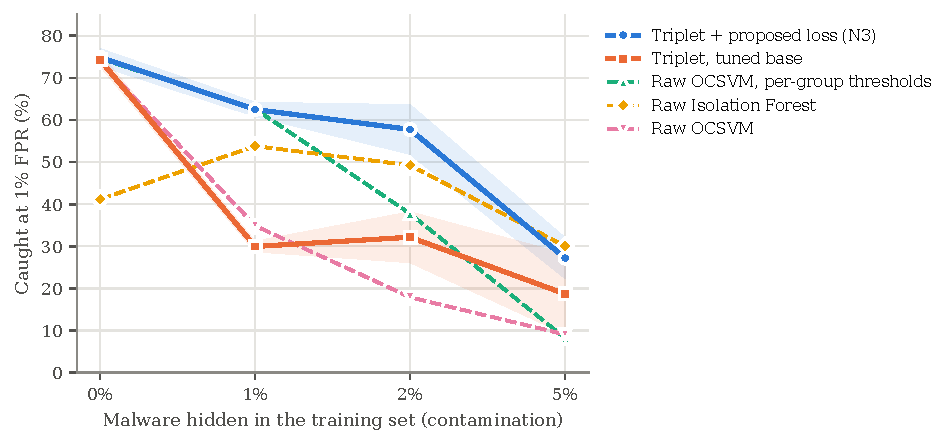
\includegraphics[width=\linewidth]{figures/fig_contamination.pdf}\caption{fig\_contamination}\end{figure}
\begin{figure}[htbp]\centering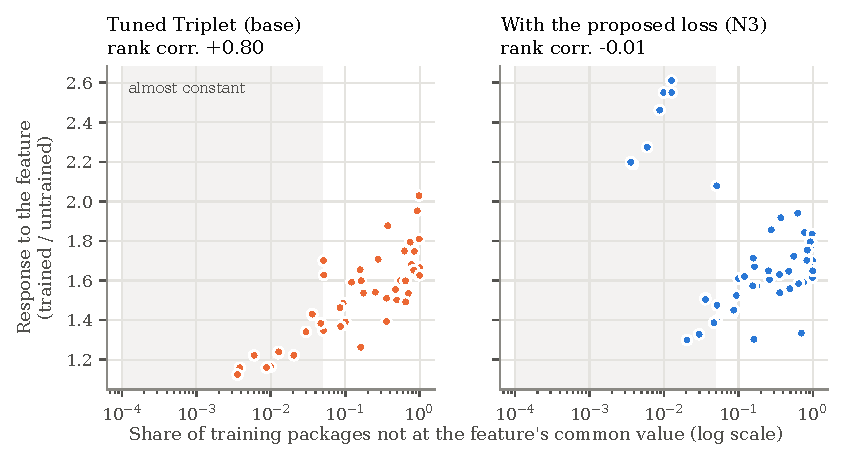
\includegraphics[width=\linewidth]{figures/fig_sensitivity.pdf}\caption{fig\_sensitivity}\end{figure}
\begin{figure}[htbp]\centering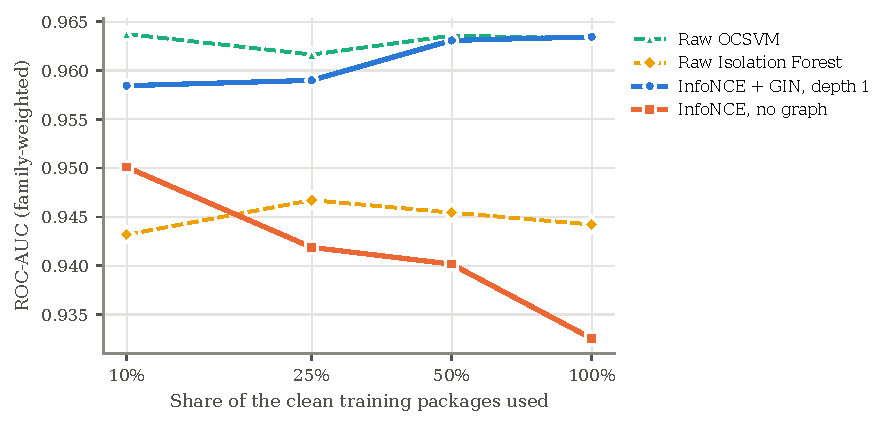
\includegraphics[width=\linewidth]{figures/fig_learning_curve.pdf}\caption{fig\_learning\_curve}\end{figure}
\begin{figure}[htbp]\centering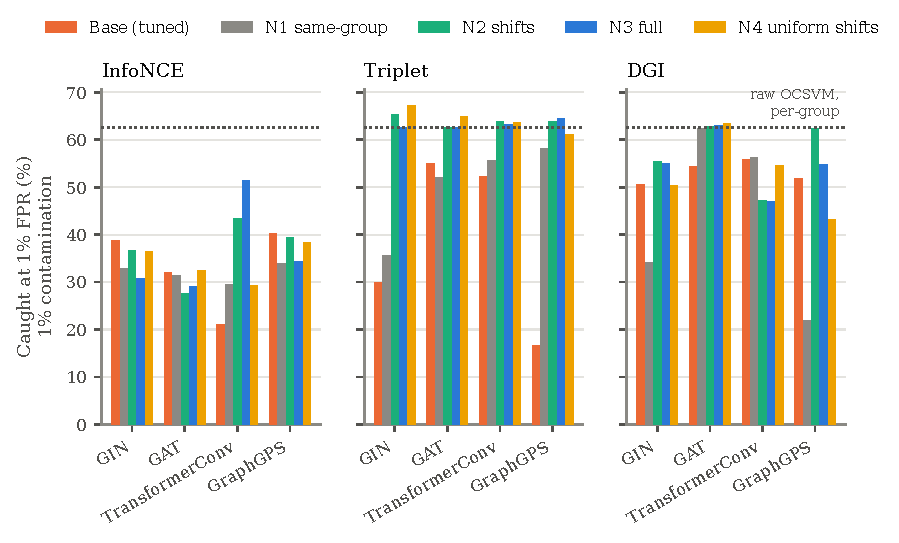
\includegraphics[width=\linewidth]{figures/fig_newloss_encoders.pdf}\caption{fig\_newloss\_encoders}\end{figure}
\end{document}
